\documentclass[]{politex}
% ========== Opções ==========
% pnumromarab - Numeração de páginas usando algarismos romanos na parte pré-textual e arábicos na parte textual
% abnttoc - Forçar paginação no sumário conforme ABNT (inclui "p." na frente das páginas)
% normalnum - Numeração contínua de figuras e tabelas 
%	(caso contrário, a numeração é reiniciada a cada capítulo)
% draftprint - Ajusta as margens para impressão de rascunhos
%	(reduz a margem interna)
% twosideprint - Ajusta as margens para impressão frente e verso
% capsec - Forçar letras maiúsculas no título das seções
% espacosimples - Documento usando espaçamento simples
% espacoduplo - Documento usando espaçamento duplo
%	(o padrão é usar espaçamento 1.5)
% times - Tenta usar a fonte Times New Roman para o corpo do texto
% noindentfirst - Não indenta o primeiro parágrafo dos capítulos/seções


% ========== Packages ==========
\usepackage[utf8]{inputenc}
\usepackage{amsmath,amsthm,amsfonts,amssymb}
\usepackage{graphicx,cite,enumerate}


% ========== Language options ==========
\usepackage[brazil]{babel}
%\usepackage[english]{babel}


% ========== ABNT (requer ABNTeX 2) ==========
%	http://www.ctan.org/tex-archive/macros/latex/contrib/abntex2
\usepackage[num]{abntex2cite}

% Forçar o abntex2 a usar [ ] nas referências ao invés de ( )
%\citebrackets{[}{]}


% ========== Lorem ipsum ==========
\usepackage{blindtext}



% ========== Opções do documento ==========
% Título
\titulo{Título}

% Autor
\autor{Lucas Arthur Felgueiras}

% Para múltiplos autores (TCC)
%\autor{Nome Sobrenome\\%
%		Nome Sobrenome\\%
%		Nome Sobrenome}

% Orientador / Coorientador
\orientador{Prof. Dr. Fabio Levy Siqueira}
% \coorientador{Nome do coorientador (opcional)}

% Tipo de documento
\tcc{Engenheiro de Computação}
%\dissertacao{Engenharia Elétrica}
%\teseDOC{Engenharia Elétrica}
%\teseLD
%\memorialLD

% Departamento e área de concentração
\departamento{Engenharia de Computação e Sistemas Digitais}
\areaConcentracao{Engenharia de Software}

% Local
\local{São Paulo}

% Ano
\data{2018}




\begin{document}
% ========== Capa e folhas de rosto ==========
\capa
\falsafolhaderosto
\folhaderosto


% ========== Folha de assinaturas (opcional) ==========
%\begin{folhadeaprovacao}
%	\assinatura{Prof.\ X}
%	\assinatura{Prof.\ Y}
%	\assinatura{Prof.\ Z}
%\end{folhadeaprovacao}


% ========== Ficha catalográfica ==========
% Fazer solicitação no site:
%	http://www.poli.usp.br/en/bibliotecas/servicos/catalogacao-na-publicacao.html


% ========== Dedicatória (opcional) ==========
\dedicatoria{Dedicatória}


% ========== Agradecimentos ==========
\begin{agradecimentos}

Thanks...

\end{agradecimentos}


% ========== Epígrafe (opcional) ==========
\epigrafe{%
	\emph{``Epígrafe''}
	\begin{flushright}
		-{}- Autor
	\end{flushright}
}


% ========== Resumo ==========
\begin{resumo}
Resumo...
%
\\[3\baselineskip]
%
\textbf{Palavras-Chave} -- Palavra, Palavra, Palavra, Palavra, Palavra.
\end{resumo}


% ========== Abstract ==========
\begin{abstract}
Abstract...
%
\\[3\baselineskip]
%
\textbf{Keywords} -- Word, Word, Word, Word, Word.
\end{abstract}


% ========== Listas (opcional) ==========
\listadefiguras
\listadetabelas

% ========== Listas definidas pelo usuário (opcional) ==========
\begin{pretextualsection}{Lista de símbolos}

Lista de símbolos...

\end{pretextualsection}

% ========== Sumário ==========
\sumario



% ========== Elementos textuais ==========

\part{Introdução}

\chapter{Objetivo}
\capepigrafe[0.5\textwidth]{First to mind when asked what 'the cloud' is, a majority respond it’s either an actual cloud, the sky, or something related to weather.}{Citrix Cloud Survey Guide\cite{quotes}}

Com o desenvolvimento da computação, novos programas foram criados, cada vez mais consumindo recursos e sendo hospedados em máquinas pessoais ou dedicadas, porém sem um gerenciamento inteligente de toda a infraestrutura. Além disso, houve a nítida migração de programas \textbf{distribuídos} pela internet para programas que \textbf{rodem} na internet.

\begin{figure}[h!]
  \centering
  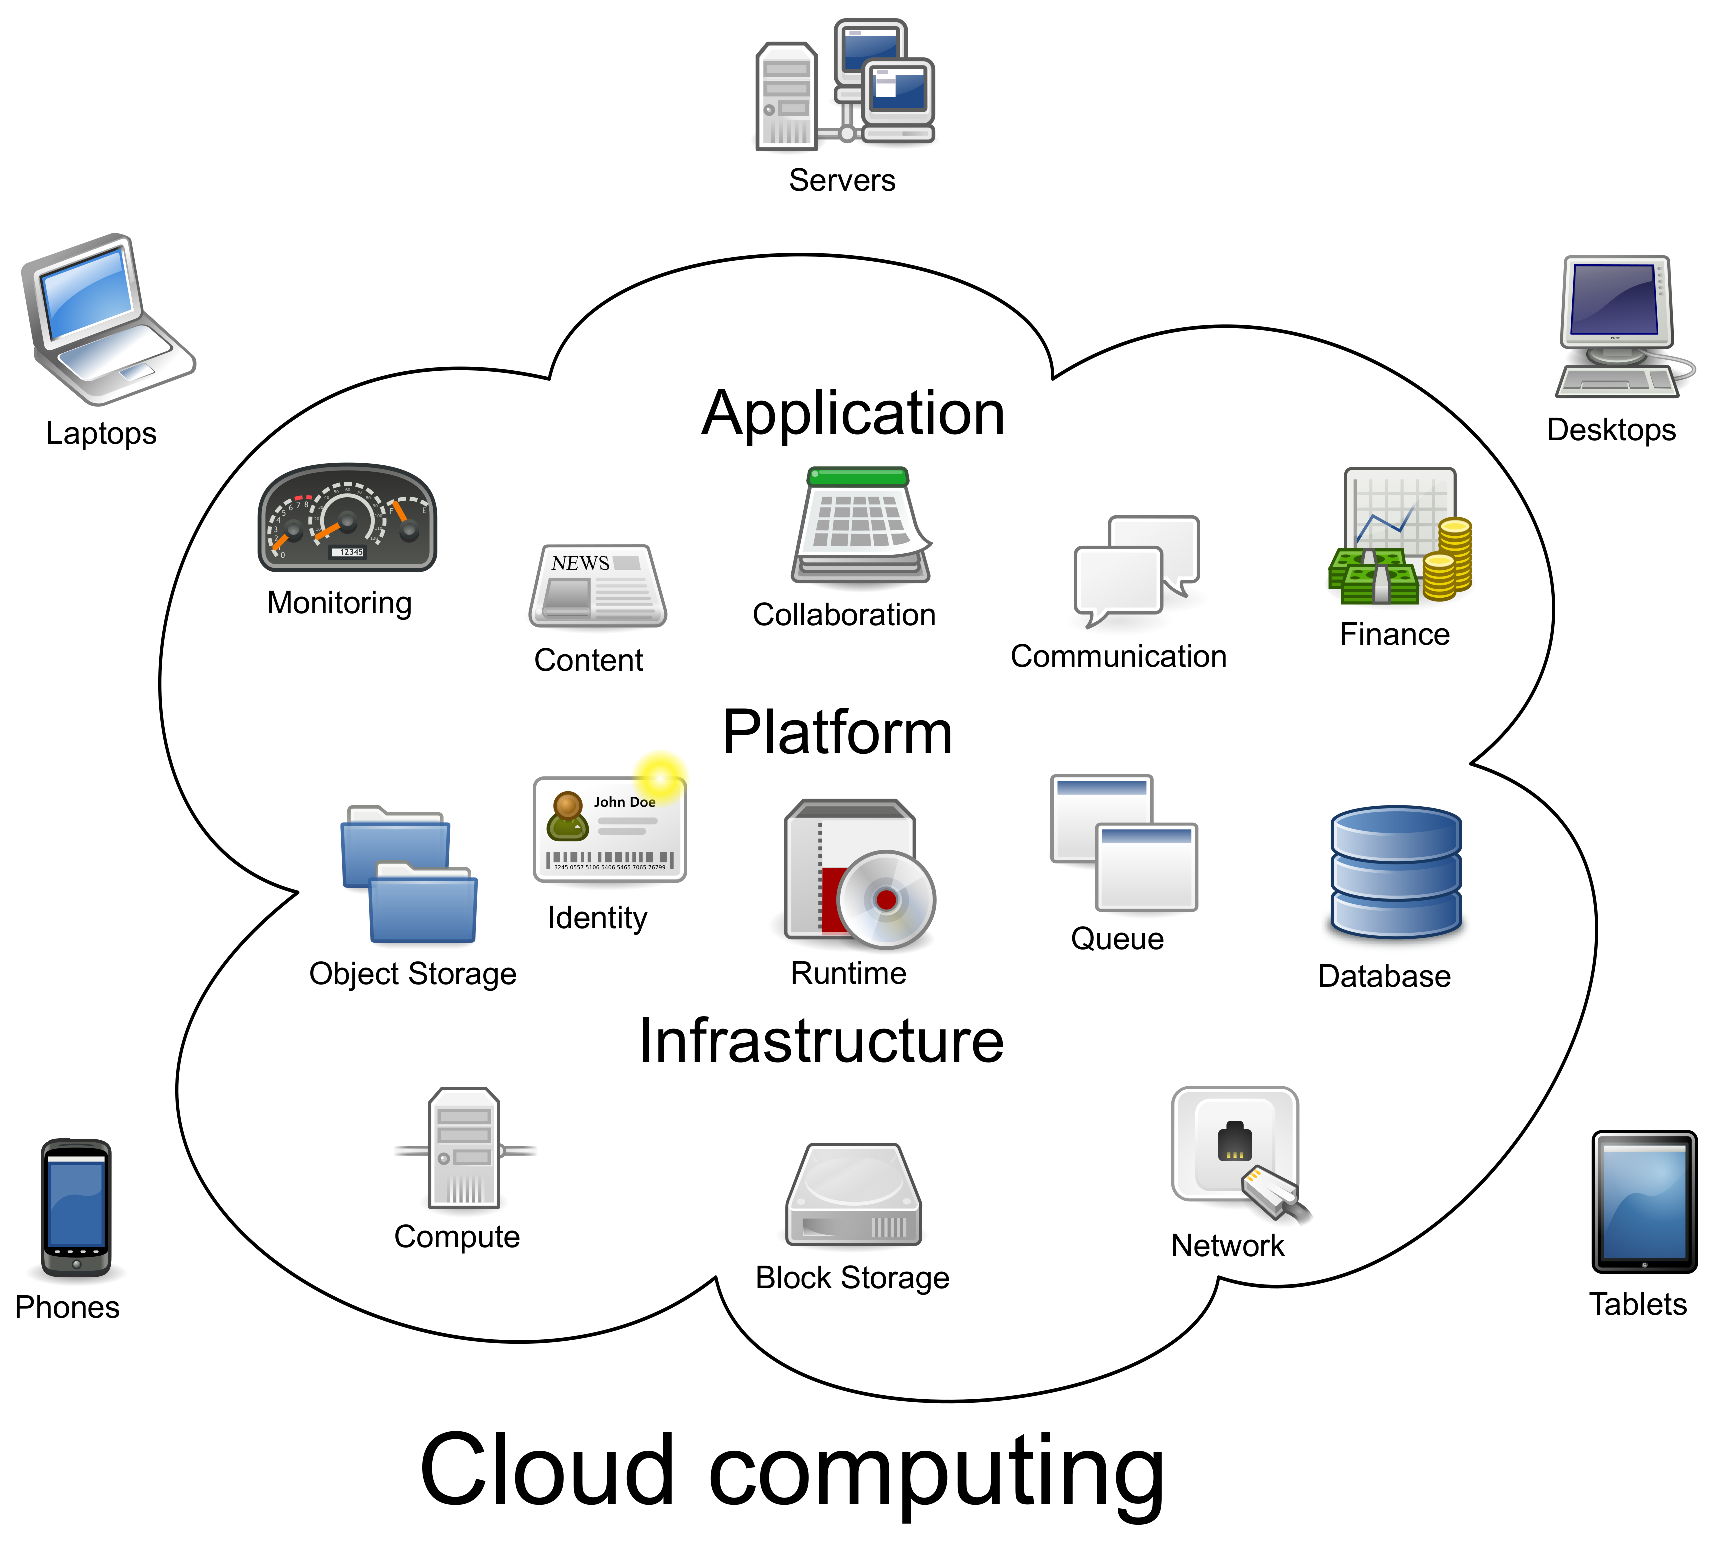
\includegraphics[scale=0.40]{imagens/cloud_computing.eps}
  \caption{Arquitetura Básica de Computação em Nuvem\cite{cloudcomputing}}
\end{figure}

Essas mudanças de paradigma motivaram a criação e consolidação do que conhecemos hoje como Computação em Nuvem, área fortalecida e necessária no desenvolvimento de programas modernos. Ao longo dos pŕoximos capítulos, haverá a explanação em detalhes de como funciona uma arquitetura em nuvem básica, seus desafios técnicos e as principais soluções existentes no mercado.

\chapter{Motivação}

\section{Contexto}
Atualmente, o gerenciamento das duas disciplinas é realizado pelo Tidia-Ae, onde apenas os professores coordenadores da disciplina podem acessar o andamento da matéria, sem a participação dos demais envolvidos, em especial dos orientadores.


\section{Problemas}
Além disso, não há um acompanhamento do status do projeto pelo Tidia-Ae, o que torna ele um simples repositório. O orientador acompanha o andamento do projeto apenas por intermédio do aluno, o que nem sempre gera uma abordagem eficiente, dado que ele depende do retorno do próprio aluno para saber atualizações, além de não ter uma central de fácil acesso para o orientador analisar os documentos relacionados.
  
Por fim, não há um sistema unificado que facilite os alunos que cursam a disciplina de consultar monografias anteriores de maneira estruturada e completamente on-line. O sistema visa, inicialmente, atacar essas demandas, de maneira a melhorar o andamento da disciplina como um todo. Futuramente, pode ser utilizada para outras disciplinas com estruturas semelhantes ao projeto de formatura.

\chapter{Justificativa}

\section{Introdução}
O departamento de Engenharia de Computação e Sistemas Digitais (PCS) da POLI possui duas matérias ao longo do último ano do curso. Cada equipe de alunos (de 1 a 3 pessoas), juntamente com um professor-orientador e um co-orientador (não-obrigatório) elabora um projeto ao longo do ano, para ser avaliado por uma banca teórica e uma feira expositiva, com a recente participação de empresas.

\section{Problemas}
Todo o processo das disciplinas é realizado de maneira manual, com exceção das entregas pontuais. Além disso, os resultados finais são publicados no site da disciplina, após os eventos de avaliação, o que dificulta, por exemplo, a avaliação das empresas. O cálculo final das médias também é manual, gerando trabalho excessivo em pouco tempo aos coordenadores.

\chapter{Organização do Trabalho}
\capepigrafe[0.5\textwidth]{``Frase espirituosa de um autor famoso''}{Autor famoso}

A equipe de desenvolvimento é composta apenas pelo aluno Lucas Arthur Felgueiras, com a orientação do Prof. Dr. Fábio Levy Siqueira, do Laboratório de Tecnologia de Software. O fato da equipe ser limitada, bem como o teor do projeto, afetou a estratégia de trabalho. Por exemplo, certas metodologias ágeis, como o \textit{Scrum}, não poderiam ser utilizadas.

\begin{citacaoLonga}
  \blindtext
\end{citacaoLonga}

\blindtext


\part{Aspectos Conceituais}

% \chapter{Casos de Uso}

\section{Introdução}
A equipe de desenvolvimento é composta apenas pelo aluno Lucas Arthur Felgueiras, com a orientação do Prof. Dr. Fábio Levy Siqueira, do Laboratório de Tecnologia de Software. O fato da equipe ser limitada, bem como o teor do projeto, afetou a estratégia de trabalho, bem como o escopo final de desenvolvimento.

\section{Problemas}
Como primeira abordagem a ser estudada para uso, escolhemos o Desenvolvimento Dirigido por Comportamento, que é uma técnica de desenvolvimento ágil que foca mais nas regras de negócio do que em detalhes técnicos em si. A princípio, seria desenvolver testes onde sua escrita seria em um nível maior do que se comparado com o Desenvolvimento Orientado a Testes.
  
Porém, um problema encontrado ao usar a abordagem citada acima seria a convergência natural ao uso de histórias de usuário, sendo essencial a participação constante das partes interessadas, o que pode dificultar o andamento do projeto. Sendo assim, descartamos seu uso, optando por linhas com a utilização de Casos de Uso.

% \chapter{Levantamento de Requisitos}
\capepigrafe[0.5\textwidth]{``Frase espirituosa de um autor famoso''}{Autor famoso}

Aqui vem o resumo do capítulo 3 do livro Use Case Modeling

\begin{citacaoLonga}
  \blindtext
\end{citacaoLonga}

\blindtext

% \include{aspectos_conceituais/continuous_delivery}

\part{Tecnologias Utilizadas}
\part{Metodologia de Trabalho}
\part{Especificação de Requisitos do Sistema}

% =========================================
\part{Projeto e Implementação}
\part{Testes e Implementação}
\part{Considerações Finais}

% \include{conclusoes_projeto_formatura}
% \include{contribuicoes}
% \include{perspectivas_continuidade}
	

% ========== Referências ==========
% --- IEEE ---
%	http://www.ctan.org/tex-archive/macros/latex/contrib/IEEEtran
%\bibliographystyle{IEEEbib}

% --- ABNT (requer ABNTeX 2) ---
%	http://www.ctan.org/tex-archive/macros/latex/contrib/abntex2
\bibliographystyle{abntex2-num}

\bibliography{}


% ========== Apêndices (opcional) ==========
\apendice
\chapter{Levantamento de Requisitos}
\capepigrafe[0.5\textwidth]{``Frase espirituosa de um autor famoso''}{Autor famoso}

Aqui vem o resumo do capítulo 3 do livro Use Case Modeling

\begin{citacaoLonga}
  \blindtext
\end{citacaoLonga}

\blindtext



% ========== Anexos (opcional) ==========
\anexo
\chapter{Documento de Visão}

\section{Introdução}
\subsection{Finalidade e Visão Geral do Documento}

O documento tem como finalidade coletar informações e unificar os pontos de vista sobre o sistema de gerenciamento da disciplina de TCC, como as necessidades encontradas e as causas para tais necessidades.

\subsection{Referências}

O site do departamento, bem como o Tidia-AE serviram como referência auxiliar para entender melhor as soluções atuais.

\section{Posicionamento}
\subsection{Descrição do Problema}

\begin{table}[!htb]
    \centering
    \caption{Descrição básica do problema}
    \label{my-label}
    \resizebox{\textwidth}{!}{\begin{tabular}{|l|l|lll}
        \cline{1-2}
        O problema de         & alto tempo e esforço para gerenciar a disciplina de maneira manual    &  &  &  \\ \cline{1-2}
        afeta                 & orientadores, alunos e coordenadores da disciplina            &  &  &  \\ \cline{1-2}
        cujo impacto é        & demora e esforço para notas, dificuldade para integração entre envolvidos, problemas de demanda     &  &  &  \\ \cline{1-2}
        uma boa solução seria & automatizar o processo e integrar os orientadores no processo &  &  &  \\ \cline{1-2}
    \end{tabular}}
\end{table}

\subsection{Sentença de Posição do Produto}

\begin{table}[!htb]
    \centering
    \caption{Sentença básica de posição do produto}
    \label{my-label}
    \resizebox{\textwidth}{!}{\begin{tabular}{|l|l|lll}
        \cline{1-2}
        Para            & alunos, orientadores, coordenadores e técnicos                                                                  &  &  &  \\ \cline{1-2}
        Que             & cursam ou estão envolvidos diretamente                                                            &  &  &  \\ \cline{1-2}
        O sistema       & de gerenciamento dos TCC's                                                                                      &  &  &  \\ \cline{1-2}
        Que             & armazena os TCC's anteriores e gerencia o TCC atual, realizando avaliação e controlando entregas                                                             &  &  &  \\ \cline{1-2}
        Ao contrário do & processo semi-manual de gerenciamento da disciplina, do Tidia-AE e do Site institucional em Wordpress                                                             &  &  &  \\ \cline{1-2}
        O sistema       & permite um acompanhamento dos envolvidos, bem como serve de histórico para os trabalhos anteriores &  &  &  \\ \cline{1-2}
    \end{tabular}}
\end{table}


\section{Descrições dos Envolvidos e Usuários}
\subsection{Resumo dos envolvidos}

Há alguns usuários que não estão diretamente envolvidos com o sistema, mas podem ser beneficiados ou interferem no sistema a ser desenvolvido:

\begin{itemize}
    \item Infraestrutura: Irá aplicar restrições tecnológicas e de negócio dado o ambiente desenvolvido.
    \item Secretaria do Departamento: Nem todos os integrantes irão usar o sistema, mas serão beneficiados pela automação de alguns processos internos da disciplina, diminuindo a demanda recorrente sobre a equipe, vide o fato deles gerenciarem as entregas das avaliações durante o processo.
\end{itemize}

\subsection{Resumo dos usuários}

Há diversos usuários que serão diretamente beneficiados com o sistema. São eles:

\begin{itemize}
    \item Coordenador: Responsáveis por administrarem as disciplinas de TCC 1 e 2 para os cursos de Engenharia de Computação Semestrais e Quadrimestrais.
    \item Orientador: Responsável por construír com os alunos a monografia.
    \item Técnico de Operação: Responsável por administrar novas funcionalidades futuras do sistema.
    \item Técnico do Evento: Responsável por cuidar da parte de infraestrutura dos eventos a serem realizados.
    \item Alunos: Os cursantes das disciplinas de TCC 1 e 2.
    \item Avaliador Teórico: Avaliam os projetos realizados, durante a banca de defesa.
    \item Avaliador Prático: Avaliam os projetos realizados, durante a feira de projetos de formatura.
\end{itemize}

\subsection{Representantes dos usuários}

Foram escolhidos representantes dos perfis citados acima, de maneira a facilitar conversas durante a especificação do documento.

\begin{itemize}
    \item João Batista/Paulo Cugnasca: Coordenadores das duas disciplinas.
    \item Edson Gomi: Professor orientador
    \item Selma: Avaliadora Teórica
    \item Nilton: Técnico do Evento
    \item Michelet: Técnico de Operação
    \item Fábio Levy: Responsável pela infraestrutura de hospedagem.
    \item Bruno Albertini: Responsável pela infraestrutura de hospedagem.
    \item Ex-aluno: Processo do lado do aluno cursante da disciplina.
\end{itemize}

\subsection{Ambiente do usuário}

Para o processo em questão, podemos reforçar alguns pontos importantes:

\begin{itemize}
    \item São 2 professores coordenadores, 2 técnicos, cerca de 50 alunos por ano de TCC e cerca de 20 professores orientadores do departamento de PCS.
    \item O ciclo da disciplinas de TCC dura 1 ano, sendo metade do tempo de especificação e metade de implementação.
    \item Atualmente, há a plataforma Tidia-AE existente para administrar as disciplinas. Porém, ela serve apenas como repositório de arquivos, sem a participação direta dos orientadores e sem infraestrutura de automação e comunicação rápida entre os envolvidos.
    \item Além disso, há o site do departamento, onde ficam as monografias mais recentes, também como simples repositório de arquivos.
\end{itemize}

\subsection{Principais necessidades do usuário}

Diversas necessidades foram encontradas, sendo agrupadas, estudadas e propostas soluções para atendê-las. A lista das necessidades encontradas está a seguir:

\begin{table}[!htb]
  \centering
  \caption{Necessidades encontradas}
  \label{my-label}
  \resizebox{\textwidth}{!}{\begin{tabular}{|l|l|l|l|}
    \hline
    Necessidade                                                                         & Prior. & Sol.Atual         & Sol. Proposta                                                \\ \hline
    Orientador, coordenadores e alunos têm dificuldades em manter contato              & 1      & E-mail, reuniões  & Colocar os orientadores nas entregas                         \\ \hline
    Busca de monografias antigas é complexa.                                            & 2      & Site do PCS       & Criar repositório de monografias finalizadas                 \\ \hline
    O processo de gerenciar empresas participantes é extremamente manual.               & 7      & Conversas         & Integrar empresas às monografias a serem avaliadas           \\ \hline
    Avaliadores têm dificuldade em acessar monografias.                                 & 4      & E-mail            & Permitir monografia de fácil acesso no sistema               \\ \hline
    Avaliação dos projetos é de maneira manual.                                         & 5      & Papel             & Permitir avaliação pelo sistema, inclusive de maneira mobile \\ \hline
    Encontrar temas e alunos e propor temas é um processo manual.                       & 9      & E-mail, conversas & Permitir alunos e orientadores proporem temas no sistema     \\ \hline
    O gerenciamento de recursos pela parte do técnico é depende dos alunos solicitarem. & 8      & E-mail, pen drive & Automatizar as demandas para os técnicos providenciarem      \\ \hline
    O processo de montagem da banca de TCC é manual.                                    & 6      & E-mail, conversas & Permitir montagem de bancas pelo sistema                     \\ \hline
    Fechar as notas finais é um processo exaustivo e com curto prazo.                   & 3      & Papel             & Automatizar o cálculo das notas finais                       \\ \hline
  \end{tabular}}
\end{table}

\subsection{Alternativas e concorrência}
\begin{itemize}
    \item Tidia-AE: Entregas pontuais, com acesso apenas aos integrantes do grupo e aos coordenadores da disciplina. Os orientadores ficam de fora das entregas principais, cabendo aos alunos realizarem essa comunicação de maneira extra-oficial.
    \item Moodle: Plataforma aberta conhecida no mercado para gerenciamento de disciplinas em geral. Serve para construir grupos e até incluir orientadores, porém não é uma alternativa simples e não possui funcionalidades de busca avançada.
    \item Site PCS (Wordpress): Apenas resultado final, de maneira pública, sem integração dos envolvidos no projeto.
\end{itemize}

\section{Visão Geral do Produto}
\subsection{Perspectiva do Produto}
O produto tem como missão automatizar o processo já existente para a disciplina, pois muitas funcionalidades propostas são realizadas de maneira manual ou simplificada, o que demanda muito tempo e esforço dos coordenadores e orientadores, tornando o processo frágil. Além disso, depende da iniciativa de todos os envolvidos, pois todo o processo de comunicação orientador-aluno é feito de maneira isolada do processo coordenador-aluno e coordenador-orientador.

\subsection{Suposições e Dependências}
A principal dependência encontrada é que o serviço deve ser hospedado na infraestrutura interna da Universidade de São Paulo, o que afetará a maneira como o produto será desenvolvido.
  
\section{Recursos do Produto}
O produto a ser desenvolvido deve atender as necessidades descritas anteriormente, ou seja, possíveis conteúdos interessantes são:

\begin{itemize}
    \item Facilitar comunicação orientador/coordenadores, permitindo que eles vejam todas as entregas dos alunos e validem, quando necessário.
    \item Buscar, de maneira pública, as monografias antigas, usando filtros e busca textual.
    \item Incluir avaliadores da feira no sistema para acompanhar monografias correntes.
    \item Permitir avaliação tanto da banca como da feira (com as empresas), permitindo acesso prévio ao conteúdo e facilitando a avaliação (de preferência na plataforma mobile).
    \item Permitir que orientadores, alunos e empresas proponham temas e consigam combinar grupos para realizar as propostas.
    \item Permitir aos técnicos gerenciarem recursos necessários para as apresentações (imprimir apresentações sem necessidade do aluno entregar arquivos via pen drive, por exemplo)
    \item Permitir a montagem de bancas de TCC, convidando os envolvidos e facilitando o acesso ao resultado final do aluno.
\end{itemize}
  
\section{Outros requisitos do produto}
Como principais requisitos não-funcionais importantes, vale ressaltar:

\begin{itemize}
    \item Confiabilidade: O sistema deve permanecer funcional durante as avaliações finais do curso, pois são cruciais para o bom andamento da matéria.
    \item Segurança: Os acessos às monografias em andamento devem ser apenas aos envolvidos diretos do trabalho. Além disso, as empresas só podem acessar o resultado final não revisado, para fins de avaliação.
    \item Usabilidade: O sistema deve ser bem intuitivo e de aprendizagem fácil, pelo tempo curto dos envolvidos na feira e pela mobilidade envolvida (avaliações pelo celular, por exemplo).
\end{itemize}

\include{anexos/diagramas_bpmn}

\end{document}
